\section{Adoption Focused Platforms} \label{chapter3:software-adoption}

The platforms previously presented focus on productivity or efficiency.
The previous section concludes that favoring one negatively impacts the other.
Moreover, a balance between productivity and efficiency is required to be both supported by the community and needed by the industry, hence trigger a virtuous circle of adoption.
Some platforms feature an abstraction of the task organization to allow developers to focus on the modular organization to keep both productivity and efficiency.
This abstraction happens either at compile time or at runtime.

% \nt{read and include \cite{Catanzaro2009} it is about Productivity language JIT compilation into efficient language
% And get all the paper that cite this one.}
% \nt{read and include \cite{Engler1994}}
% \nt{read and include \cite{Kovachev2011}}
% \nt{read and include \cite{Asanovic2006}}

\begin{figure}[h!]
\textfig{%
  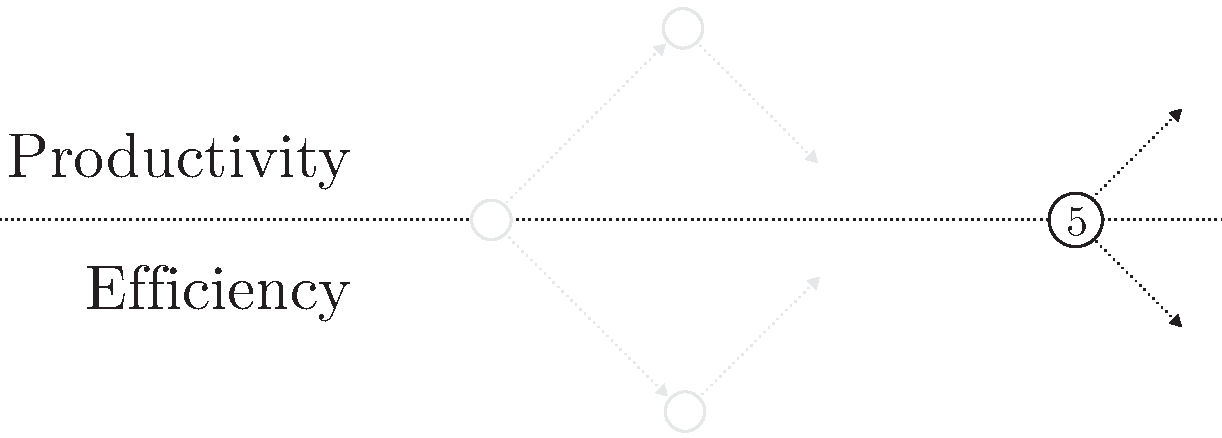
\includegraphics[width=0.6\textwidth]{../resources/state-of-the-art-5.pdf}%
  \caption{Focus on Adoption}%
  \label{fig:state-of-the-art-5}%
}%
\end{figure}

\subsection{Abstraction of Tasks Organization}

\subsubsection{Compilers} \label{chapter3:software-adoption:compilers}

\cit{It is a mistake to attempt high concurrency without help from the compiler.}{R. Behren, J. Condit, E. Brewer \cite{Behren2003}}

The idea to bridge the gap between the tasks and modules organizations dates from the initial paper that presented this gap \cite{Parnas1972}.
However, the implementation of this idea remains a work in progress.

% read and include \cite{Catanzaro2009}

\paragraph{Parallelism Extraction}

To extract parallelism from a sequential implementation, a compiler needs to identify the commutative operations to parallelize their executions \cite{Rinard1996,Clements2013a}.
The parallelization of loop iterations has been thoroughly studied \cite{Mauras1989,Amarasinghe1995,Chen2008,Banerjee2013,Radoi2014}, particularly with the polyhedral compilation method \cite{Bastoul2004}.
Examples of polyhedral compilers are \ImplementationsOf{Polyhedral Compilers}.
To improve performance gains outside of loops, some compilers identify parallelism in the data-flow representation on the whole program \cite{Beck1991,Catanzaro2009,Li2012}.

Data processing applications \cite{Fernandez2014a} such as web services \cite{Salmito2013} are often already organized as data-flow.
In higher-order programming, continuous passing style and promises encourage this data-flow organization.
However, the mutable closures required for higher-order programming remains a challenge to parallelize because they rely on a globally shared memory \cite{Harrison1989, Nicolay2010, Matsakis2012a}.
To extract parallelism, compilers rely on static analysis or notations from the developers.

% TODO Extract parallelism compilers from these :
% Load balanced pipeline parallelism \cite{Kamruzzaman2013},
% Regent \cite{Slaughter2015},
% Cilk-P, On-the-Fly Pipeline Parallelism\cite{Lee2013}
% Commutativity analysis: A new analysis framework for parallelizing compilers \cite{Rinard1996}
% Introducing 'Bones': a parallelizing source-to-source compiler based on algorithmic skeletons \cite{Nugteren2012}
% \cite{Herrmann2000}

\paragraph{Static analysis}

Compilers analyze the source code of a program to detect commutative operations in the control flow \cite{Allen1970}.
The point-to analysis is a static analysis method.
It identifies multiple symbolic names pointing to the same memory location.
That is called aliasing.
Hence it idenfities side-effects \cite{Andersen1994,Jang2009,Sridharan2012,Wei2014} between operations, which allows to infer their commutativity.
Another method, the abstract interpretation, is to interpret the possible path of executions with virtual inputs.
It allows to statically reason on the behavior of dynamic programs \cite{Maffeis2008,Smith2011,Gardner2012,Hackett2012,Raychev2013,Gardner2013,Bodin2014}.
It is successfully used for security applications to detect malicious scripts, or obfuscate code \cite{Huang2004,Jovanovic2006,Yu2007,Maffeis2009a,Chudnov2015,Dolby2015}
% \nt{Update the citation for Dolby2015}.

However, these static analysis methods remains often too imprecise, and expensive for the performance gain to be profitable in dynamic languages, such as Javascript \cite{Shivers1991}.
Instead, some compilers relies on annotations from the developers.

\paragraph{Annotations}

Some works proposed to rely on annotations from the developer to identify the shared data structures and infer the commutativity of operations \cite{Vandierendonck2010a,Fernandez2014a}.
Such annotations are especially relevant for accelerators such as GPUs or FPGAs, because the development effort yields huge performance improvements \cite{Tarditi2006}.
Examples of such compilers are \ImplementationsOf{Annotation Compilers}.

% Bloom declarative language \ftnt{http://bloom-lang.net/}
% Blazes: Coordination analysis for distributed programs \cite{Alvaro2014}

\paragraph{Compilation Limitations}

For dynamic languages like Javascript, the static analysis is not sufficient to correctly infer the independence of tasks to parallelize them.
Parallel compilers often fall back on relying on annotations provided by developers.
Hence, the burden of detailing the tasks and memory organizations falls back to the developer.
It impacts productivity and adoption.

\subsubsection{Runtimes} \label{chapter3:software-adoption:runtimes}

At runtime, the incertitudes on the independence of tasks is resolved.
It allows analyzes precise enough to detect and distribute the commutative operations.

\paragraph{Partitioned Global Address Space}

The Partitioned Global Address Space (PGAS) provides a uniform access on a distributed memory architecture.
It attempts to combine the efficiency of distributed memory systems, with the productivity of shared memory systems.
Each computing node executes the same program, and provides its local memory to be shared with all the other nodes.
The PGAS platform assures the remote accesses and synchronization of memory across nodes.
Examples of implementations of the PGAS model are \ImplementationsOf{Partitioned Global Address Space}.

\paragraph{Dynamic Distribution of Execution}

Following SEDA, Leda proposes a model where the independent stages of the pipeline are defined only by their role in the application \cite{Salmito2013,Salmito2014}.
The execution distribution and module organization are different.
The actual execution distribution is defined automatically during deployment.
This automation manages the execution organizations to help the developer focus on the modular organization.
% However, it doesn't improve the composition of module with higher-order programming.

\subsubsection{Productivity and Efficiency}

The platforms presented in this section intend to merge both productivity and efficiency in a single platform by bringing parallelism to productivity languages.
Because they are based on productivity languages, they feature decent encapsulation, but they limit the use of higher-order programming between tasks to allow their isolation.
Hence, it degrades composition, as presented in table \ref{tab:adoption-productivity}.

Despite worse productivity, this parallelization bring good efficiency, as presented in table \ref{tab:adoption-efficiency}.

\AbstractionProductivityTable{tab:adoption-productivity}
\AbstractionEfficiencyTable{tab:adoption-efficiency}

\subsection{Limitation}

The platforms presented in this section come from the need of the industry to reduce the development commitment required for efficiency.
However, these platforms respond exclusively to academic or industrial needs, and are barely supported by the community, as presented in table \ref{tab:adoption-efficiency}.

The balance between efficiency and productivity is not sufficient for a community of passionate to arise.
To be largely adopted, the platforms need to allow novice to start learning and experimenting at small scale.
It incites the community to start projects, and grow them organically to build businesses.
The context of web development is particularly adapted for this growth.

\AbstractionAdoptionTable{tab:adoption-efficiency}

\subsection{Summary}

As detaild in table \ref{tab:adoption-summary}, this section proved that a platform cannot trade productivity against efficiency without massively losing the community required to trigger the adoption.

\AbstractionSummaryTable{tab:adoption-summary}











\endinput
